% Options for packages loaded elsewhere
\PassOptionsToPackage{unicode}{hyperref}
\PassOptionsToPackage{hyphens}{url}
\PassOptionsToPackage{dvipsnames,svgnames,x11names}{xcolor}
%
\documentclass[
  letterpaper,
  DIV=11,
  numbers=noendperiod]{scrartcl}

\usepackage{amsmath,amssymb}
\usepackage{lmodern}
\usepackage{iftex}
\ifPDFTeX
  \usepackage[T1]{fontenc}
  \usepackage[utf8]{inputenc}
  \usepackage{textcomp} % provide euro and other symbols
\else % if luatex or xetex
  \usepackage{unicode-math}
  \defaultfontfeatures{Scale=MatchLowercase}
  \defaultfontfeatures[\rmfamily]{Ligatures=TeX,Scale=1}
\fi
% Use upquote if available, for straight quotes in verbatim environments
\IfFileExists{upquote.sty}{\usepackage{upquote}}{}
\IfFileExists{microtype.sty}{% use microtype if available
  \usepackage[]{microtype}
  \UseMicrotypeSet[protrusion]{basicmath} % disable protrusion for tt fonts
}{}
\makeatletter
\@ifundefined{KOMAClassName}{% if non-KOMA class
  \IfFileExists{parskip.sty}{%
    \usepackage{parskip}
  }{% else
    \setlength{\parindent}{0pt}
    \setlength{\parskip}{6pt plus 2pt minus 1pt}}
}{% if KOMA class
  \KOMAoptions{parskip=half}}
\makeatother
\usepackage{xcolor}
\setlength{\emergencystretch}{3em} % prevent overfull lines
\setcounter{secnumdepth}{-\maxdimen} % remove section numbering
% Make \paragraph and \subparagraph free-standing
\ifx\paragraph\undefined\else
  \let\oldparagraph\paragraph
  \renewcommand{\paragraph}[1]{\oldparagraph{#1}\mbox{}}
\fi
\ifx\subparagraph\undefined\else
  \let\oldsubparagraph\subparagraph
  \renewcommand{\subparagraph}[1]{\oldsubparagraph{#1}\mbox{}}
\fi


\providecommand{\tightlist}{%
  \setlength{\itemsep}{0pt}\setlength{\parskip}{0pt}}\usepackage{longtable,booktabs,array}
\usepackage{calc} % for calculating minipage widths
% Correct order of tables after \paragraph or \subparagraph
\usepackage{etoolbox}
\makeatletter
\patchcmd\longtable{\par}{\if@noskipsec\mbox{}\fi\par}{}{}
\makeatother
% Allow footnotes in longtable head/foot
\IfFileExists{footnotehyper.sty}{\usepackage{footnotehyper}}{\usepackage{footnote}}
\makesavenoteenv{longtable}
\usepackage{graphicx}
\makeatletter
\def\maxwidth{\ifdim\Gin@nat@width>\linewidth\linewidth\else\Gin@nat@width\fi}
\def\maxheight{\ifdim\Gin@nat@height>\textheight\textheight\else\Gin@nat@height\fi}
\makeatother
% Scale images if necessary, so that they will not overflow the page
% margins by default, and it is still possible to overwrite the defaults
% using explicit options in \includegraphics[width, height, ...]{}
\setkeys{Gin}{width=\maxwidth,height=\maxheight,keepaspectratio}
% Set default figure placement to htbp
\makeatletter
\def\fps@figure{htbp}
\makeatother

\KOMAoption{captions}{tableheading}
\makeatletter
\makeatother
\makeatletter
\makeatother
\makeatletter
\@ifpackageloaded{caption}{}{\usepackage{caption}}
\AtBeginDocument{%
\ifdefined\contentsname
  \renewcommand*\contentsname{Table of contents}
\else
  \newcommand\contentsname{Table of contents}
\fi
\ifdefined\listfigurename
  \renewcommand*\listfigurename{List of Figures}
\else
  \newcommand\listfigurename{List of Figures}
\fi
\ifdefined\listtablename
  \renewcommand*\listtablename{List of Tables}
\else
  \newcommand\listtablename{List of Tables}
\fi
\ifdefined\figurename
  \renewcommand*\figurename{Figure}
\else
  \newcommand\figurename{Figure}
\fi
\ifdefined\tablename
  \renewcommand*\tablename{Table}
\else
  \newcommand\tablename{Table}
\fi
}
\@ifpackageloaded{float}{}{\usepackage{float}}
\floatstyle{ruled}
\@ifundefined{c@chapter}{\newfloat{codelisting}{h}{lop}}{\newfloat{codelisting}{h}{lop}[chapter]}
\floatname{codelisting}{Listing}
\newcommand*\listoflistings{\listof{codelisting}{List of Listings}}
\makeatother
\makeatletter
\@ifpackageloaded{caption}{}{\usepackage{caption}}
\@ifpackageloaded{subcaption}{}{\usepackage{subcaption}}
\makeatother
\makeatletter
\@ifpackageloaded{tcolorbox}{}{\usepackage[many]{tcolorbox}}
\makeatother
\makeatletter
\@ifundefined{shadecolor}{\definecolor{shadecolor}{rgb}{.97, .97, .97}}
\makeatother
\makeatletter
\makeatother
\ifLuaTeX
  \usepackage{selnolig}  % disable illegal ligatures
\fi
\IfFileExists{bookmark.sty}{\usepackage{bookmark}}{\usepackage{hyperref}}
\IfFileExists{xurl.sty}{\usepackage{xurl}}{} % add URL line breaks if available
\urlstyle{same} % disable monospaced font for URLs
\hypersetup{
  colorlinks=true,
  linkcolor={blue},
  filecolor={Maroon},
  citecolor={Blue},
  urlcolor={blue},
  pdfcreator={LaTeX via pandoc}}

\author{}
\date{}

\begin{document}
\ifdefined\Shaded\renewenvironment{Shaded}{\begin{tcolorbox}[sharp corners, boxrule=0pt, breakable, frame hidden, interior hidden, enhanced, borderline west={3pt}{0pt}{shadecolor}]}{\end{tcolorbox}}\fi

Caleb Skinner

Global Health Survey Questions 6-10

\hypertarget{questions}{%
\subsection{Questions:}\label{questions}}

\hypertarget{in-your-opinion-are-there-enough-global-health-opportunities-available-to-us-pre-medical-students}{%
\subsection{6. In your opinion, are there enough global health
opportunities available to US pre-medical
students?}\label{in-your-opinion-are-there-enough-global-health-opportunities-available-to-us-pre-medical-students}}

A. Overall Results for Global Health Opportunities Availability.

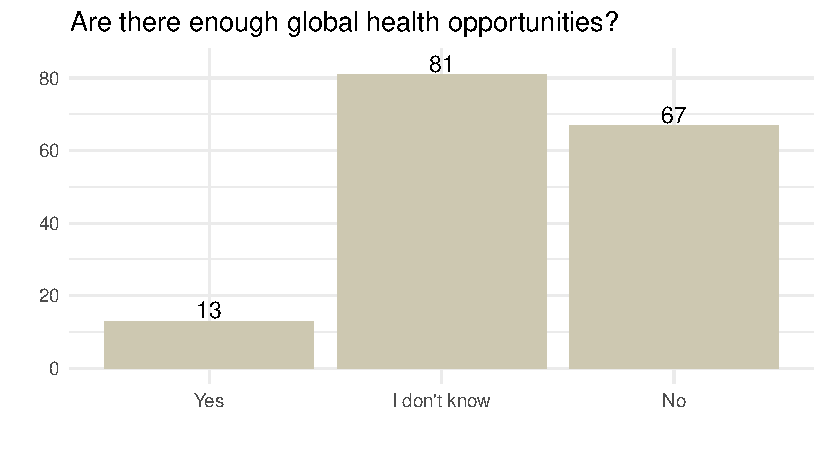
\includegraphics{GlobalHealthQuarto6-10_files/figure-pdf/unnamed-chunk-2-1.pdf}

\newpage

B. Global Health Opportunities by Global Health Career Interest

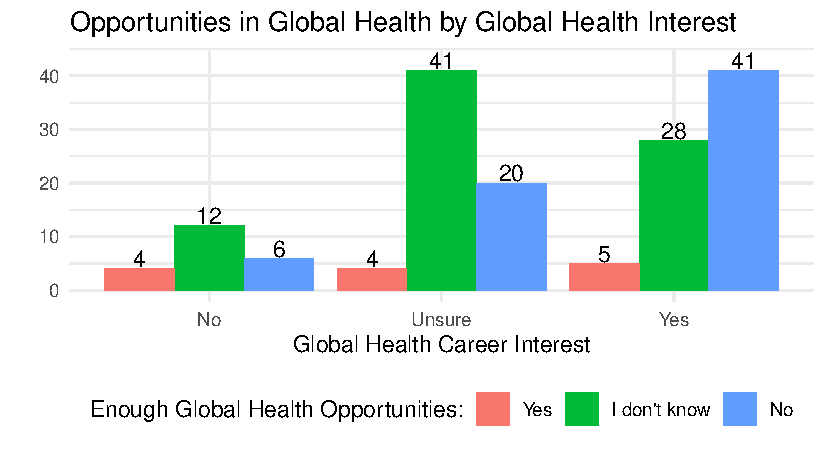
\includegraphics{GlobalHealthQuarto6-10_files/figure-pdf/unnamed-chunk-3-1.pdf}

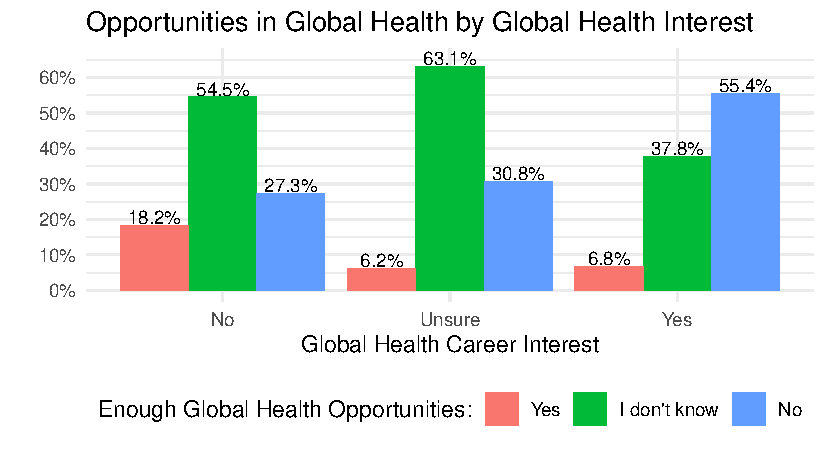
\includegraphics{GlobalHealthQuarto6-10_files/figure-pdf/unnamed-chunk-4-1.pdf}

\newpage

The following is a t-test measuring the difference in belief that there
are sufficient Global Health opportunities for pre-med students in those
who have expressed interest in a Global Health Career and those who have
not. For this t-test, I counted ``I don't know'' responses to the
sufficient Global Health Opportunities Question as 1/2 a ``yes'' and 1/2
a ``no''. The results are significant. Those who have express an
interest in a Global Health Career indicate that there are not
sufficient Global Health Opportunities at a higher rate than those who
have not expressed an interest in a Global Health Career.

\begin{verbatim}
# 
#   Welch Two Sample t-test
# 
# data:  df18ttest %>% filter(Q14 == "No") %>% select(Q18) and df18ttest %>% filter(Q14 == "Yes") %>% select(Q18)
# t = 2.4289, df = 32.145, p-value = 0.02091
# alternative hypothesis: true difference in means is not equal to 0
# 95 percent confidence interval:
#  0.03194622 0.36363118
# sample estimates:
# mean of x mean of y 
# 0.4545455 0.2567568
\end{verbatim}

The following is a second t-test measuring the difference in belief that
there are sufficient Global Health opportunities for pre-med students in
those who have expressed interest in a Global Health Career and those
who have not. For this t-test, I removed all ``I don't know'' responses.
The results are not significant. This is likely because a large amount
of respondents selected ``I don't know.'' This drops the sample size to
only 80.

\begin{verbatim}
# 
#   Welch Two Sample t-test
# 
# data:  df18ttest %>% filter(Q14 == "No", Q18 != 0.5) %>% select(Q18) and df18ttest %>% filter(Q14 == "Yes", Q18 != 0.5) %>% select(Q18)
# t = 1.7159, df = 10.498, p-value = 0.1155
# alternative hypothesis: true difference in means is not equal to 0
# 95 percent confidence interval:
#  -0.08453279  0.66714149
# sample estimates:
# mean of x mean of y 
# 0.4000000 0.1086957
\end{verbatim}

\newpage

\hypertarget{which-if-any-of-the-following-do-you-perceive-as-reasons-it-is-difficult-for-undergraduate-pre-medical-students-to-learn-more-about-global-health-and-gain-experience-in-the-field-prior-to-medical-school}{%
\subsection{7. Which, if any, of the following do you perceive as
reasons it is difficult for undergraduate pre-medical students to learn
more about global health and gain experience in the field prior to
medical
school?}\label{which-if-any-of-the-following-do-you-perceive-as-reasons-it-is-difficult-for-undergraduate-pre-medical-students-to-learn-more-about-global-health-and-gain-experience-in-the-field-prior-to-medical-school}}

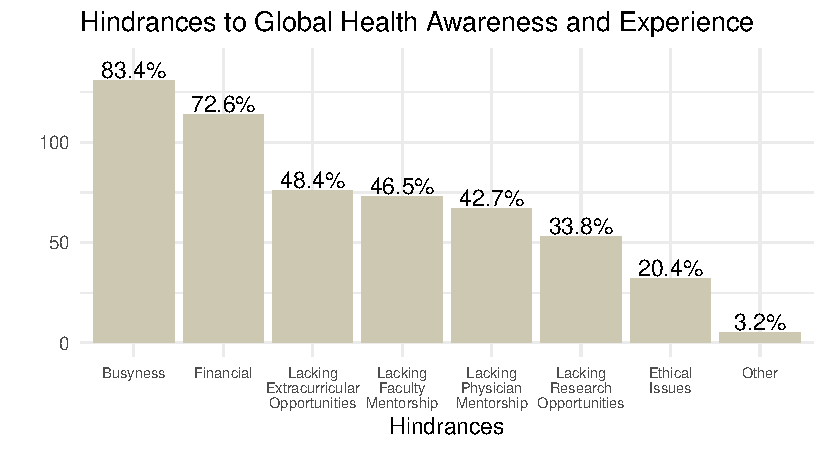
\includegraphics{GlobalHealthQuarto6-10_files/figure-pdf/unnamed-chunk-7-1.pdf}

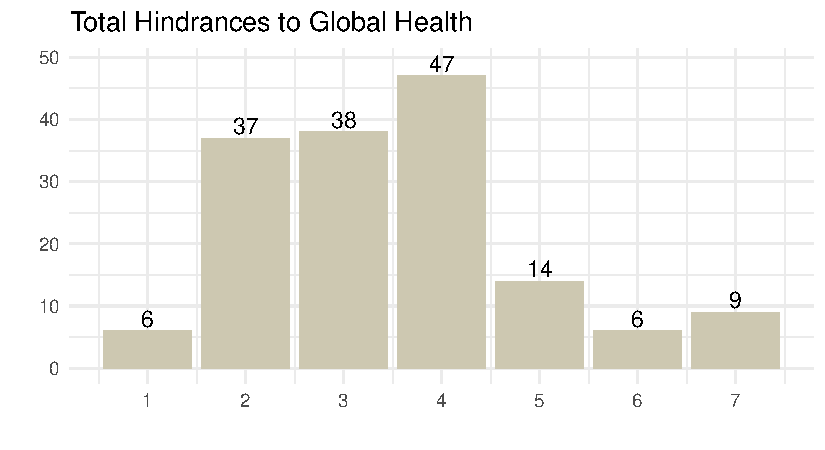
\includegraphics{GlobalHealthQuarto6-10_files/figure-pdf/unnamed-chunk-8-1.pdf}

\newpage

\hypertarget{what-do-you-think-should-be-required-for-pre-medical-students-to-engage-in-clinical-global-health-work-andor-mission-trips}{%
\subsection{8. What do you think should be required for pre-medical
students to engage in clinical global health work and/or mission
trips?}\label{what-do-you-think-should-be-required-for-pre-medical-students-to-engage-in-clinical-global-health-work-andor-mission-trips}}

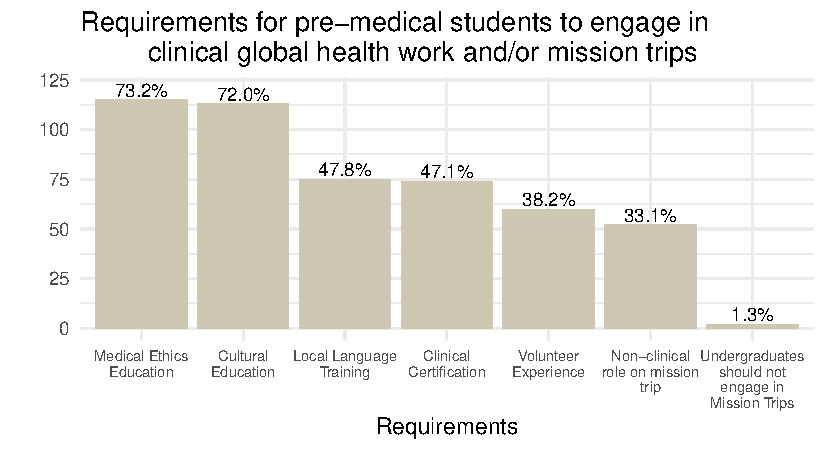
\includegraphics{GlobalHealthQuarto6-10_files/figure-pdf/unnamed-chunk-9-1.pdf}

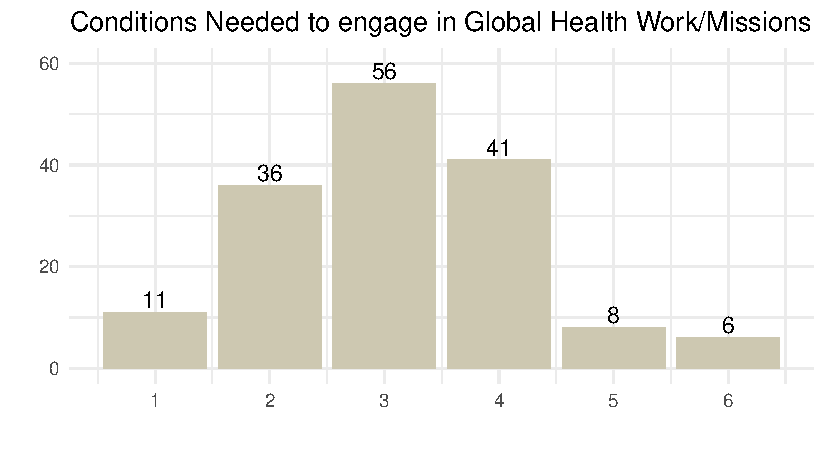
\includegraphics{GlobalHealthQuarto6-10_files/figure-pdf/unnamed-chunk-10-1.pdf}

\newpage

\hypertarget{short-term-mission-trips-are-an-effective-way-to-address-global-health-challenges.}{%
\subsection{9. Short-term mission trips are an effective way to address
global health
challenges.}\label{short-term-mission-trips-are-an-effective-way-to-address-global-health-challenges.}}

A. Overall Results

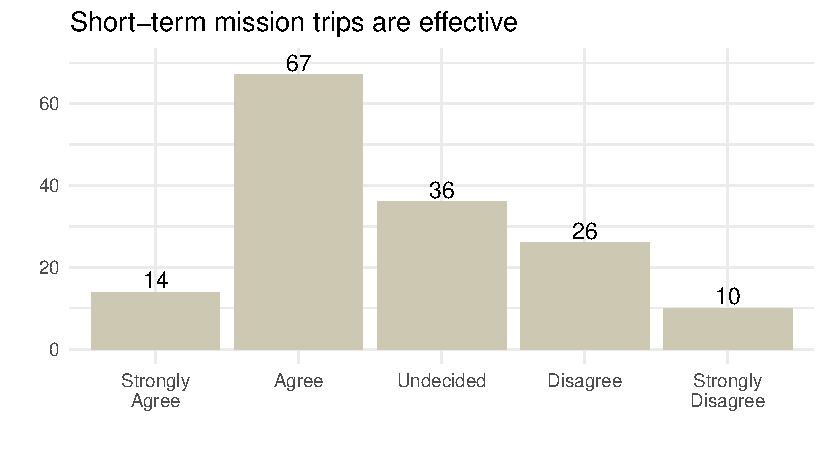
\includegraphics{GlobalHealthQuarto6-10_files/figure-pdf/unnamed-chunk-11-1.pdf}

\newpage

B. Effectiveness of Mission Trips by Lived Abroad

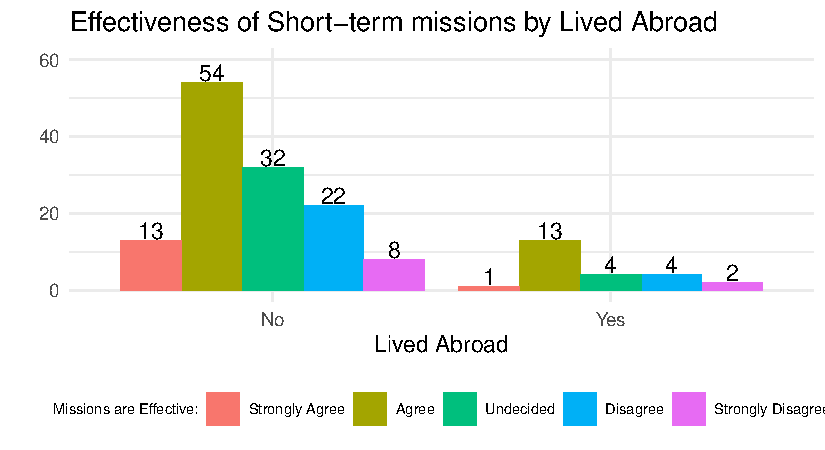
\includegraphics{GlobalHealthQuarto6-10_files/figure-pdf/unnamed-chunk-12-1.pdf}

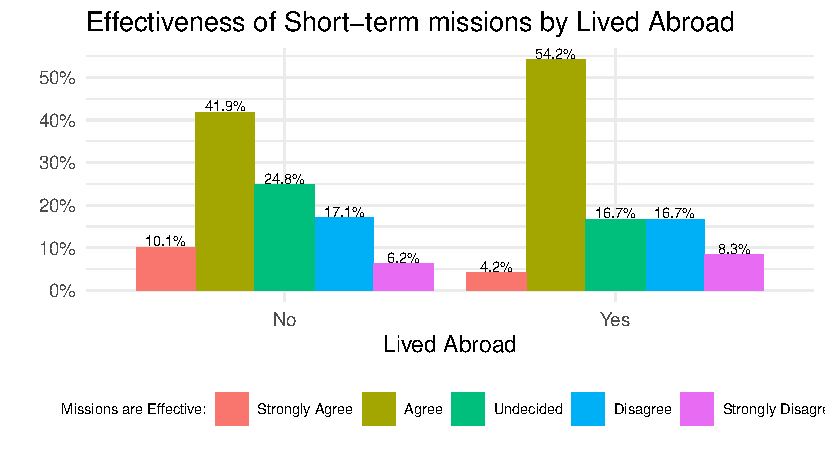
\includegraphics{GlobalHealthQuarto6-10_files/figure-pdf/unnamed-chunk-13-1.pdf}

\newpage

C. Effectiveness of Mission Trips by Born Abroad

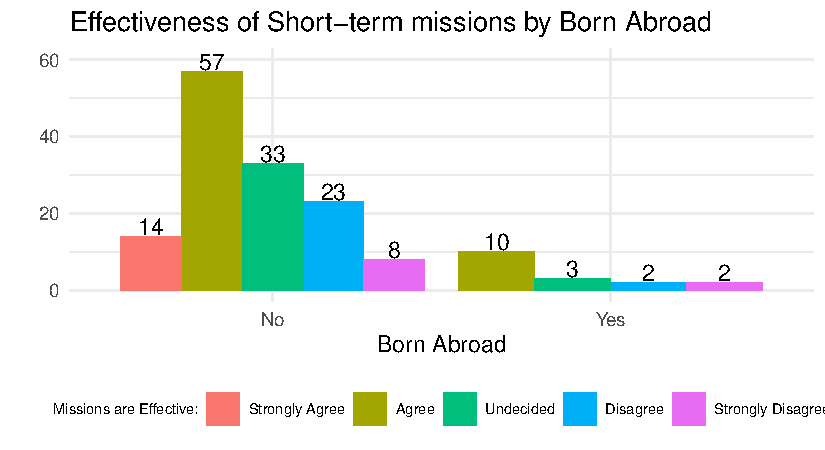
\includegraphics{GlobalHealthQuarto6-10_files/figure-pdf/unnamed-chunk-14-1.pdf}

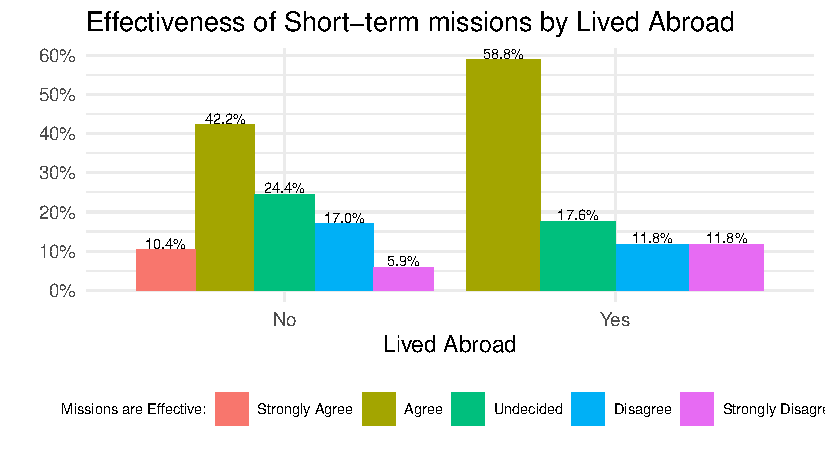
\includegraphics{GlobalHealthQuarto6-10_files/figure-pdf/unnamed-chunk-15-1.pdf}

\newpage

\hypertarget{practicing-clinical-medicine-is-the-most-important-aspect-of-global-health.}{%
\subsection{10. Practicing clinical medicine is the most important
aspect of global
health.}\label{practicing-clinical-medicine-is-the-most-important-aspect-of-global-health.}}

A. Overall Results

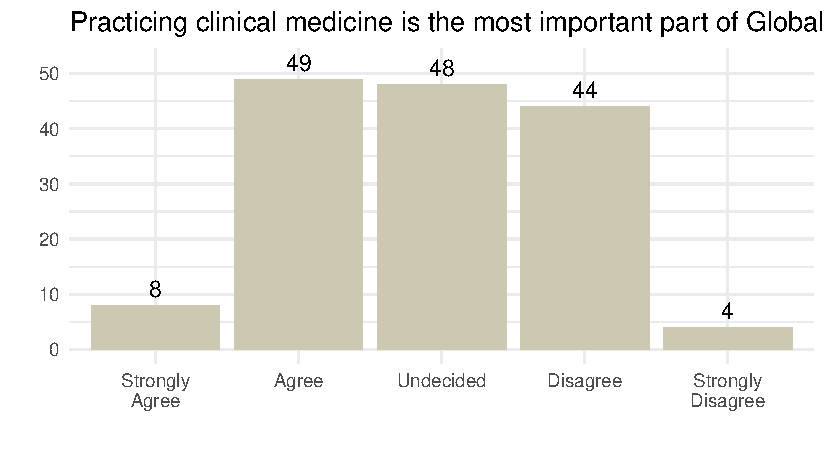
\includegraphics{GlobalHealthQuarto6-10_files/figure-pdf/unnamed-chunk-16-1.pdf}

\newpage

B. Importance of Clinical Medicine by Major

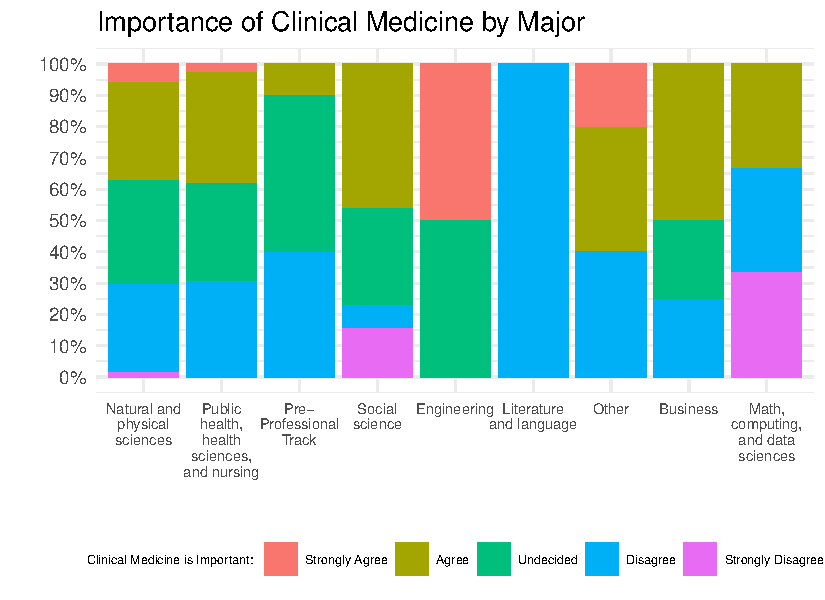
\includegraphics{GlobalHealthQuarto6-10_files/figure-pdf/unnamed-chunk-17-1.pdf}

\newpage

C. Importance of Clinical Medicine by Global Health Interest

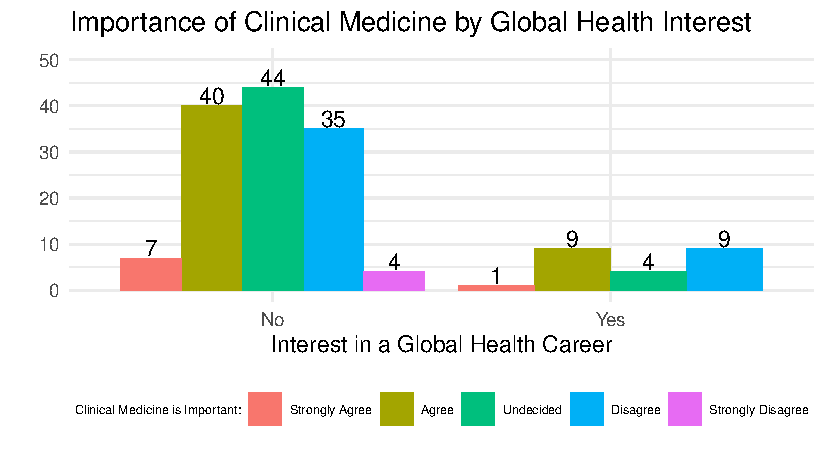
\includegraphics{GlobalHealthQuarto6-10_files/figure-pdf/unnamed-chunk-18-1.pdf}

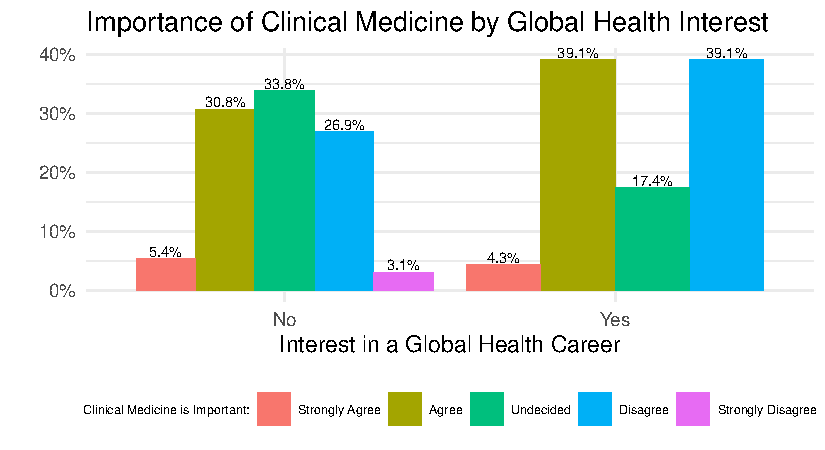
\includegraphics{GlobalHealthQuarto6-10_files/figure-pdf/unnamed-chunk-19-1.pdf}



\end{document}
